\section{Implementation procedure} \label{sec:imp-procedure}

To implement the features listed in \charef{cha:design}, a stepwise approach was utilised. First, the finished design concept was cut into modules, each with a clearly defined, separate task to accomplish. These modules are what constitutes the final product, however it is possible to implement each of them independently of the others. The modules were ordered according to their importance and relevance to the final product's overall quality, and then tested and implemented in the order seen below.

\begin{enumerate}
\item Basic movement
\item Object collection
\item Bluetooth communication
\item Boundary detection
\item Object detection
\item Basic object navigation
\item Advanced movement
\item Advanced route navigation
\end{enumerate}

This approach made it possible to ensure, that a new feature or module of the robot would only be implemented, when the robot's previously implemented modules are fully operational and complete. This means that each module is known to be working correctly, the challenge is then to combine these. 

This should not be viewed as an absolute approach: work did begin on the next iterations, even if the prior ones weren't finished yet, however it serves well to illustrate how the process was planned and in what order the features were added.

To visualise these modules, a flowchart tool was used to map the different actions and considerations the robot makes when complete. Each added module of functionality was assigned with a new colour to maintain an overview of the iterations. 

\begin{figure}[H]
     \center{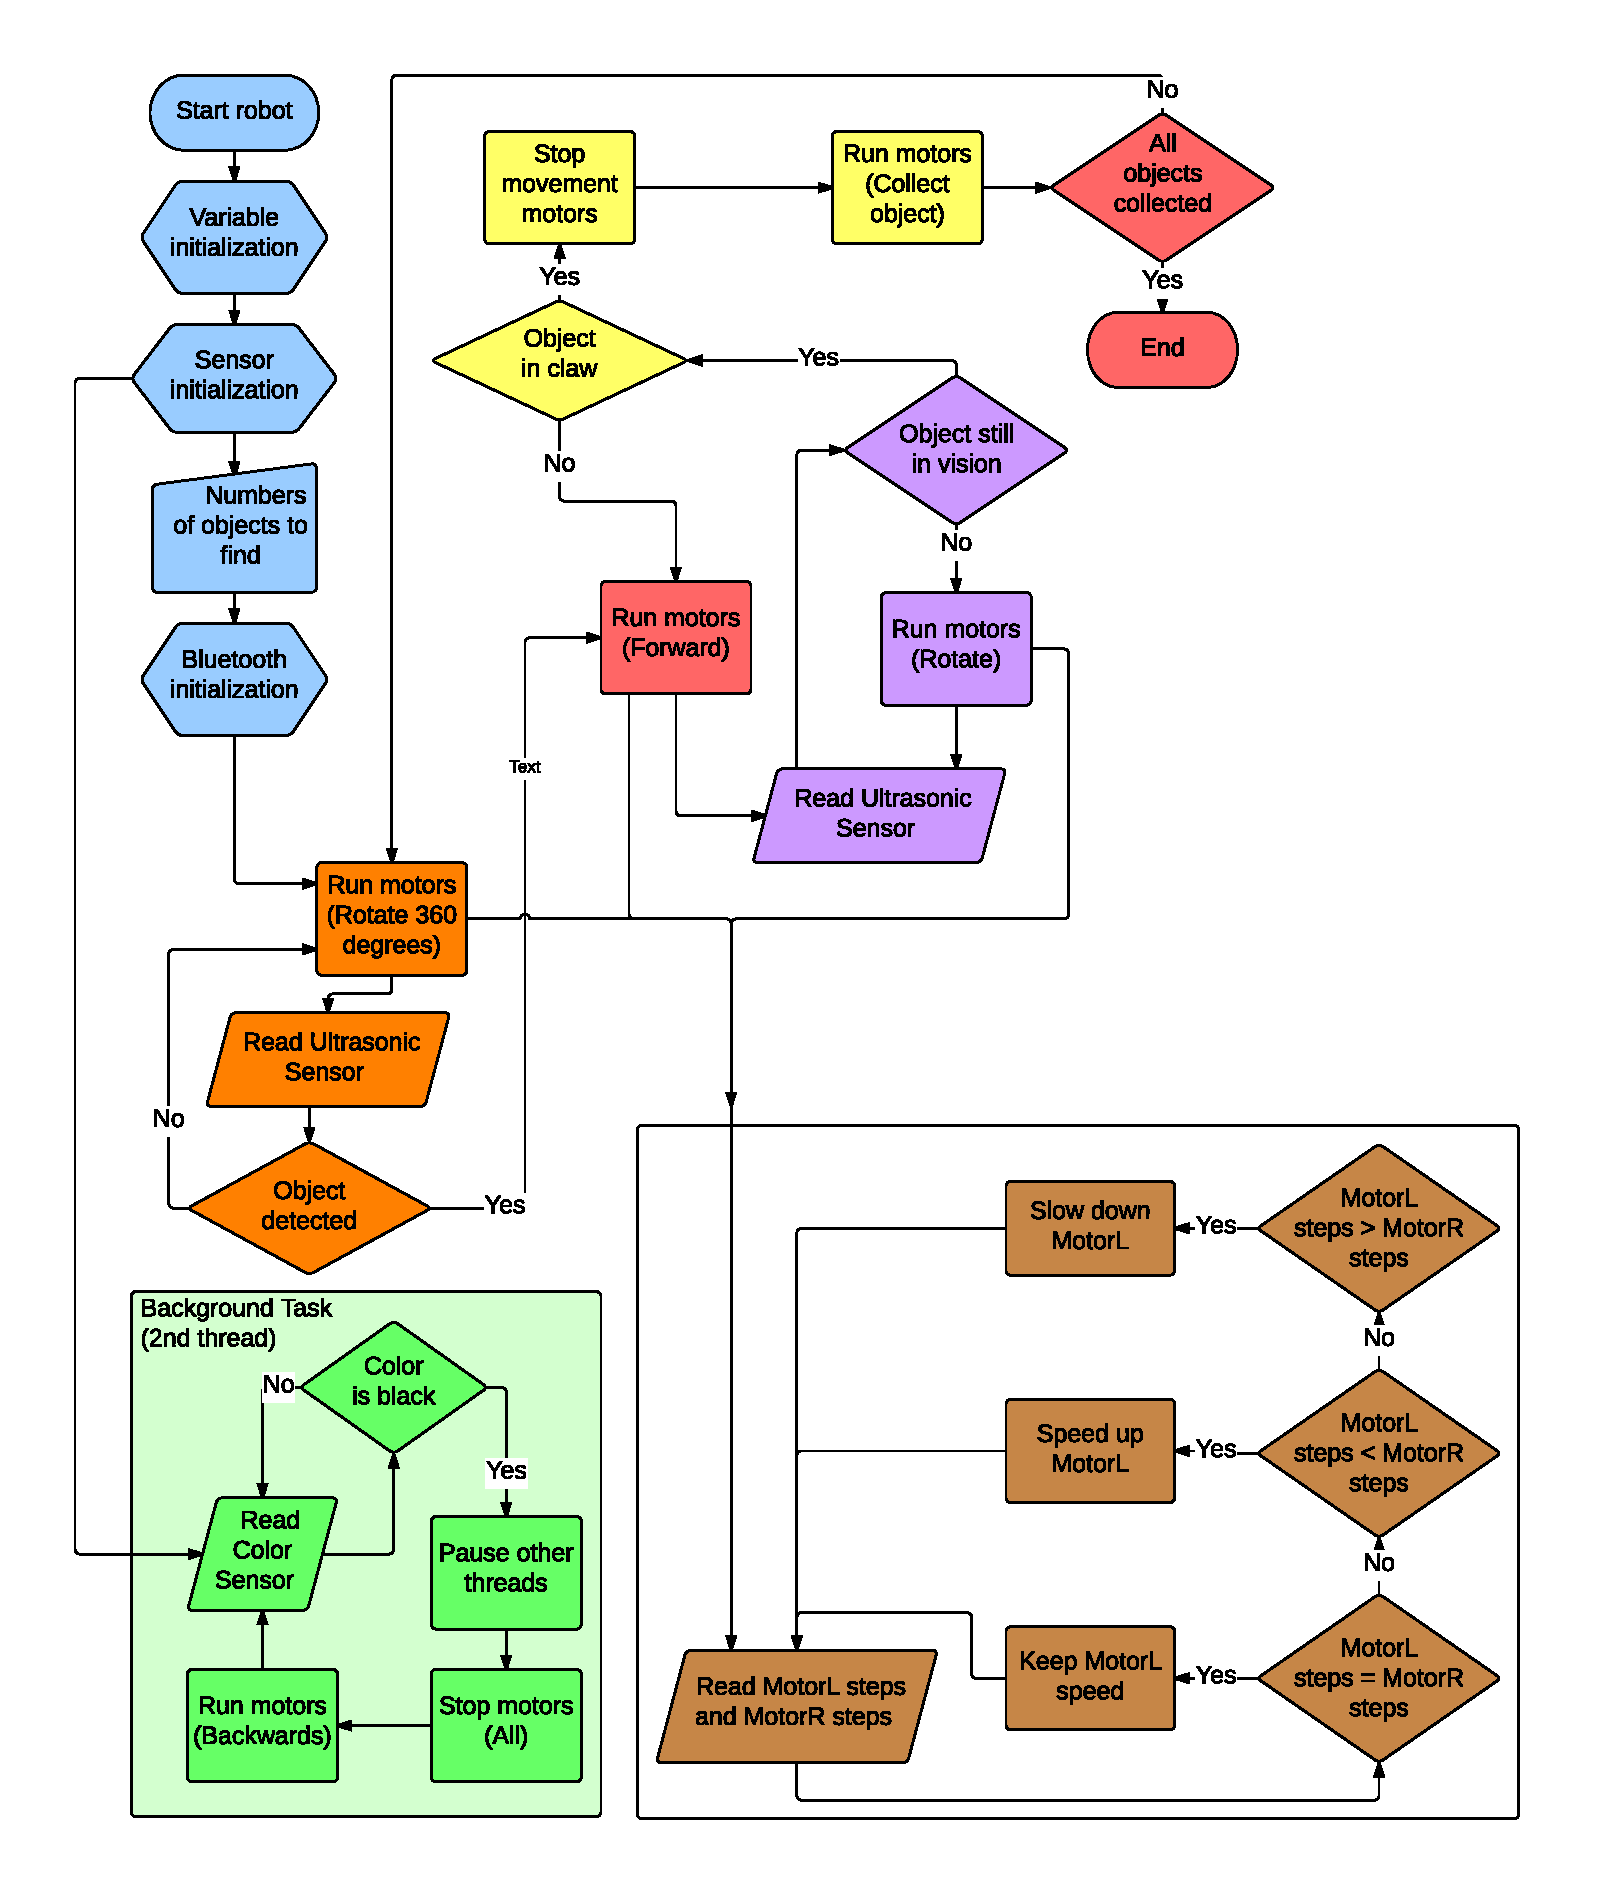
\includegraphics[width=\textwidth]
     {graphics/CompleteRobotFlowchart.pdf}}
     \caption{\label{fig:CompleteRobotFlowchart} Flowchart of the robot and its behaviour.}
\end{figure}
\fxnote{Skal vi tilføje tekst til MC boksen?}

In the diagram in \figref{fig:CompleteRobotFlowchart}, the sections are coloured according to what functionality they fulfil. The previously mentioned iterations often focus on one of the particular partitions of the flowchart. The iterations are described below.


\subsubsection{First iteration --- Basic movement}
In the first iteration, the first module was implemented: the basic movement behaviour. This iteration resulted in a basic robot with tank treads, that could move forward and backwards, and turn left and right around its own vertical axis. The robot, at this point, was able to move around in a square pattern, and end up at the starting location, with an accuracy of a few centimetres. Movement accuracy at this point was hard coded. The blue part in \figref{fig:CompleteRobotFlowchart}, which is the basis for all implementation, was also implemented in this iteration, except for the bluetooth initialisation.


\subsubsection{Second iteration --- Object collection}
In the second iteration, the robotic arm and claw used to collect objects were designed, built and developed. This collection module was tested and tweaked separately, after which it was implemented into the robot itself. This module corresponds to the yellow part in \figref{fig:CompleteRobotFlowchart}.


\subsubsection{Third iteration --- Bluetooth communication}
With the \projname{} being able to move, controlled by one of the NXT brick, and a claw and arm capable of collecting objects controlled by another brick, communication between these two bricks was the next priority to implement. This was done using the inherent Bluetooth-capabilities of the bricks. The master brick sends instructions to the slave brick, and await confirmation from the slave brick, when the task is done. This allowed for the code and behaviour to be centralised on one brick, only communicating simple instructions once in a while over Bluetooth.


\subsubsection{Fourth iteration --- Boundary detection}
This iteration implemented the colour sensors, and made it possible to detect the environment boundaries. This includes functionality to stop, reverse, and turn away from the detected line, searching for new objects. This entire feature runs in a thread by itself. This corresponds to the green part in \figref{fig:CompleteRobotFlowchart}. 


\subsubsection{Fifth iteration --- Object detection}
This iteration included the implementation of basic object detection; the \projname{} is at this point able to turn 360 degrees around while scanning for objects with the ultrasonic sensor. The ultrasonic sensor is able to detect the distance between the robot and the target object. This corresponds to some of the states in the orange part in \figref{fig:CompleteRobotFlowchart}.


\subsubsection{Sixth iteration --- Object navigation}
This iteration focused on implementing the next-in-view algorithm to find and collect objects within the boundary. The routine to find lost objects, as described in \secref{sec:niv-algorithm}, can be seen in \figref{fig:CompleteRobotFlowchart} as the purple part.


\subsubsection{Seventh iteration --- Advanced movement}
During this iteration a motor controller was developed, to ensure that the motors drive alike, in the amount of steps driven. This motor controller is used to drive straight forwards and backwards with greater precision, than the basic movement it replaces. Another motor controller was developed, but this one is used to turn the \projname{} with precision. This motor controller is used to turn a given amount of degrees, or get to a heading, choosing the most relevant turning direction. This feature is shown in the brown part in \figref{fig:CompleteRobotFlowchart}.


\subsubsection{Eight iteration --- Advanced route navigation}
The last iteration was supposed to implement the NN-algorithm described in \secref{sec:nn-algorithm}, but due to the result of the hardware test, it was decided not to implement the NN-algorithm in the final version. The ultrasonic sensor was not able to detect objects with enough precision so that the \projname{} could accurately calculate any useful information based on the data. Due to this limitation, the \emph{next-in-view} algorithm was chosen for implementation. The source code of the NN-algorithm can be found in \appref{app:CD}.


%The hardware problems, primarily the ones caused by the ultrasonic sensor, were too difficult to solve at this point in the project and this iteration will therefore not be implemented in the final program. Instead, the next-in-view algorithm will be the final algorithm. It is possible to see what would have been implemented in \secref{sec:object-navigation}. A comparison between algorithms, and a more detailed explanation of them, can be seen in \secref{sec:algorithm-desc}.

%The blue section, with the \emph{Start robot} node, is the initial start-up phase of the robot. Variables and sensors are initialised, and the number of objects to look for is determined through user input. This is the basis for the implementation. The parts marked in red describe the behaviour of the movement module. The initial implementation of the movement was the ability to move forwards, backwards and to turn left and right with some precision. The yellow part is the object collection behaviour, which handles the movement of the claw and arm that grab hold of and then collect the objects in the environment. After the arm and claw could successfully grab and collect objects, it was implemented into the movement module, to prevent the robot from changing position while an object is being collected.

%Afterwards, the purple part --- the object-detecting half of the scanning module --- was implemented, to allow the robot to actually detect the objects and determine when to activate the collection module. This module also guides the movement module's behaviour, since the movement at this stage is based on where the 

%one brick being the master unit sending instructions, the other being the slave, receiving instructions and returning confirmation. In the case of \projname{}, the brick with the scanners and the movement control was chosen to be the master, and the brick in control of the object collection module the slave. This allowed for the code and behaviour to be centralised on one brick, only communicating simple instructions once in a while over Bluetooth. 

%This iteration focus on implementing a more intelligent way to locate and collect all objects. At this point the robot is able to locate all the visible objects from the starting position. The robot turn 360 degrees and save the angle and distance of all the objects which the robot detects. The \projname{} then navigates to the spotted objects in sequence and attempts to grab these. If the boundary is spotted while driving to a object, then the \projname{} abandons the object, and moves on to the next object. 

%moving towards any object spotted. When it is within sufficient range of the object, it will attempt to pick up the object using the previously implemented collection module. This basic object detection allows the robot to --- in some cases --- complete the intended task successfully.